\documentclass{beamer}
\mode<presentation>
{
  \usetheme{default}      % or try Darmstadt, Madrid, Warsaw, ...
  \usecolortheme{default} % or try albatross, beaver, crane, ...
  \usefonttheme{default}  % or try serif, structurebold, ...
  \setbeamertemplate{navigation symbols}{}
  \setbeamertemplate{caption}[numbered]
} 
\usepackage{amsmath}
\usepackage[portuguese]{babel}
\usepackage[utf8x]{inputenc}

\title[Linear Model]{Modelos Lineares}
\author{Otaviano da Cruz Neto}
\institute{Instituto de Ciencias Exatas - ICEX / UFF }
\date{06/06/2018}

\begin{document}

\begin{frame}
  \titlepage
\end{frame}
\section{Introducao}
\begin{frame}{Introdução}
\begin{itemize}
\item \textbf{O que é o método de Regressão?}

O método de Regressão é uma ferramenta que leva em consideração a dependência entre as variáveis que caracterizam os dados . Ou seja, a cada valor de entrada é associado a um valor dado por uma Função Target, o padrão a ser aprendido.

\item \textbf{Tipos de Regressão}\\
Os dois tipos de regressão que serão exibidos serão a Regressão Linear e a Regressão Logística. A regressão linear admite a dependência linear entre as variáveis e busca um hiperplano que melhor aproxima a configuração. Já a regressão logística utiliza a associação de cada conjunto de características a respostas binárias, por exemplo, 0 ou 1.    
\end{itemize}
\end{frame}
\begin{frame}{Introdução}

\begin{itemize}
  
  \item \textbf{Dados Individuais ($X^{(i)}$,$Y^{(i)}$)}
  \begin{equation}
  X^{(i)} = \left[  x_1, x_2, \cdots, x_m \right] 
  \end{equation}
  \begin{equation}
  Y^{(i)} = y^{(i)}  
  \end{equation}
  \item \textbf{Dados da Amostra (X e Y)}
  \begin{equation}
 X = \left[ \begin{array}{rrccccrr}
1 &&& x_1^{(1)} && \cdots && x_m^{(1)} \\ 
1 &&& x_1^{(2)} && \cdots && x_m^{(2)} \\
\vdots &&& \vdots && \cdots && \vdots \\
1 &&& x_1^{(N)} && \cdots && x_m^{(N)} 

\end{array} \right]
  \end{equation}
  \end{itemize}
  \end{frame}
  
  \begin{frame}{Introdução} 
  	\begin{equation}
  	Y = \left[
    	\begin{array}{rrcrr}
    	y^{(1)}\\
        y^{(2)}\\
        \vdots \\
        y^{(N)}
    	\end{array}
    	\right]
  	\end{equation}
  \end{frame}

\section{Regressão Linear}

\begin{frame}{Regressão Linear}

\begin{itemize}
  \item \textbf{Vetor Normal à Hipótese}
  \begin{equation}
  W = \left[w_0, w_1, w_2, \cdots, w_m\right]
  \end{equation}
  \item \textbf{Hipótese Linear}
 \begin{equation}
 h(w) = X W^T
 \end{equation}
 
 \item \textbf{Caracterização do Erro dentro ($E_{in}$) da amostra}\\
 A preocupação com o erro que envolve o aprendizado de um padrão é evidente já que há a necessidade de aplicar em outros juntos fora da amostragem. Neste caso temos,  
\begin{equation}
E_{in}(W) = \frac{1}{N} \sum_{n = 1}^N \left( X^{(n)}  W^T - Y^{(n)} \right)^2 = \frac{1}{N} \left( XW^T -Y\right)^2 
\end{equation}
\end{itemize}
\end{frame}



\begin{frame}{Regressão Linear}
\begin{itemize}
\item \textbf{Gradiente de $E_{in}$ $\left(\vec{\nabla} E_{in}\right)$}

\begin{equation}
\vec{\nabla} E_{in} = \frac{2}{N} X^T \left( XW^T - Y \right)
\end{equation}
 \item  \textbf{ Gradiente descedente (Solução Numérica)} : O método do gradiente decrescente é uma ferramenta que utiliza a propriedade do operador gradiente de apontar sempre na direção de máximo crescimento, afim de minimizar o erro dentro da amostra.
 \begin{equation}
 \vec{W}_{t+1} = \vec{W}_t -  \alpha \vec{\nabla} E_{in}
 \end{equation}
\end{itemize}
\end{frame} 

\begin{frame}{Regressão Linear}
\begin{figure}
\centering
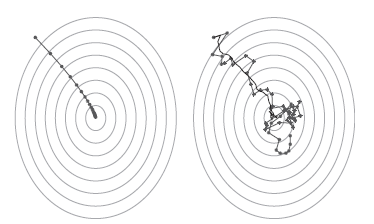
\includegraphics[width = 0.7\textwidth]{Gradiente.png}
\caption{Diferença de valores de passos e suas convergência.}
\end{figure}
\end{frame}
 
 \section{Solução}
 
 \begin{frame}{Solução da Regressão Linear}
 
 \begin{itemize}
 \item \textbf{ Normalização (Solução analítica)}
 \begin{equation}
 \vec{\nabla} E_{in} = \frac{2}{N} X^T \left( XW^T - Y \right) = 0
 \end{equation}
 \begin{equation}
	 W^T = X^{\dagger} Y
 \end{equation}
 \begin{equation}
 X^{\dagger} = \left( X^T X \right)^{-1} X^T
 \end{equation}
 \item \textbf{ Regressão Linear e PLA( Hipótese Inicial )}\\
 Muitas vezes na aplicação do Perceptron Learning Algorithm é inicialmente estipulado os valores do vetor normal (W) de maneira aleatória, e , por isso, pode haver uma demora em relação à convergência do algoritmo. Assim, afim de evitar tal situação, iniciar com uma hipótese que caracteriza melhor a amostragem é uma boa estratégia para diminuir o tempo de convergência. Ou seja, aplicando o algoritmo de regressão linear na amostragem e, a partir do padrão da regressão, aplicar o PLA. 
 \end{itemize}
 \end{frame}
 
 \begin{frame}{Regressão Linear}
\begin{itemize}
\item \textbf{Visualização Gráfica}
\begin{figure}
\centering
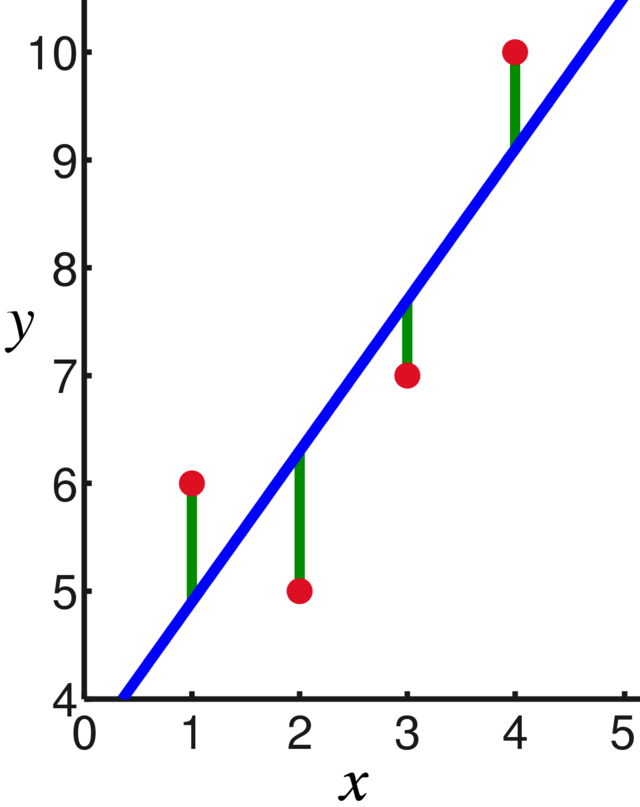
\includegraphics[width=0.55\textwidth]{MinimizarError.png}
\end{figure}
\end{itemize}
\end{frame}
 
 \begin{frame}{Interpretação Probabilística}
 \begin{itemize}
 \item \textbf{ Gaussiana (IID - Independente e identicamente distribuidos)}\\
 Tomando que 
 \begin{equation}
 Y^{(i)} = X^{(i)}W^T + \epsilon_i
 \end{equation}
 Podemos expressar $\epsilon_i \approx N(0,\sigma ^2)$ , então a densidade de $\epsilon_i$ é dada por:
 \begin{equation}
 p(\epsilon_i) = \frac{2}{\sqrt[]{2 \pi} \sigma} exp \left( - \frac{(Y^{(i)} - X^{(i)}W^T)^2}{2 \sigma ^2} \right)
 \end{equation}
 Então a probabilidade(Likelihood) da Hipótese Linear é:
 \begin{equation}
 L(W) = \prod_{i=1} ^N \frac{2}{\sqrt[]{2 \pi} \sigma} exp \left( - \frac{(Y^{(i)} - X^{(i)}W^T)^2}{2 \sigma ^2} \right)
 \end{equation}
 \end{itemize}
 \end{frame}
 
\begin{frame}{Interpretação Probabilística}
É fundamental diferenciar os papeis das duas expressões (14 e 15), respectivamente. Na equação 14 tem-se a probabilidade individual dentro da amostra em função de $Y^{(i)}$ fixando W. Já na 15 temos a probabilidade geral da amostra em função de W, pois é justamente o valor de W que determinará o erro da amostra como um todo. 
\begin{equation}
L(W) = L(W;X,Y) = p(Y|X;W)
\end{equation}
 Então derivando o $ \ln L(w) $ temos:
 \begin{equation}
 l(W) = \ln L(w)
 \end{equation}
 
 \begin{equation}
 	=\ln \prod_{i=1} ^N \frac{2}{\sqrt[]{2 \pi} \sigma} exp \left( - \frac{(Y^{(i)} - X^{(i)}W^T)^2}{2 \sigma ^2} \right)
 \end{equation}
     \end{frame}
     
  \begin{frame}{Interpretação Probabilística}
   \begin{equation}
  = \sum_{i=1}^N \ln  \frac{2}{\sqrt[]{2 \pi} \sigma} exp{ \left( - \frac{(Y^{(i)} - X^{(i)}W^T)^2}{2 \sigma ^2} \right)}
 \end{equation} 
 
 \begin{equation} 
 =  N\ln \frac{1}{\sqrt[]{2 \pi} \sigma} - \frac{1}{\sigma ^2 }  \frac{1}{2}\sum_{i=1}^N \left(    	Y^{(i)} - X^{(i)}W^T \right)^2
    \end{equation}
  Maximizando temos:
  \begin{equation}
   l(W) = \frac{1}{2}\sum_{i=1}^N \left(Y^{(i)} - X^{(i)}W^T \right)^2
  \end{equation}
  \end{frame}
  
  \begin{frame}{Aplicação}
  \begin{itemize}
  \item \textbf{ Dados}
  \begin{figure}
  \centering
  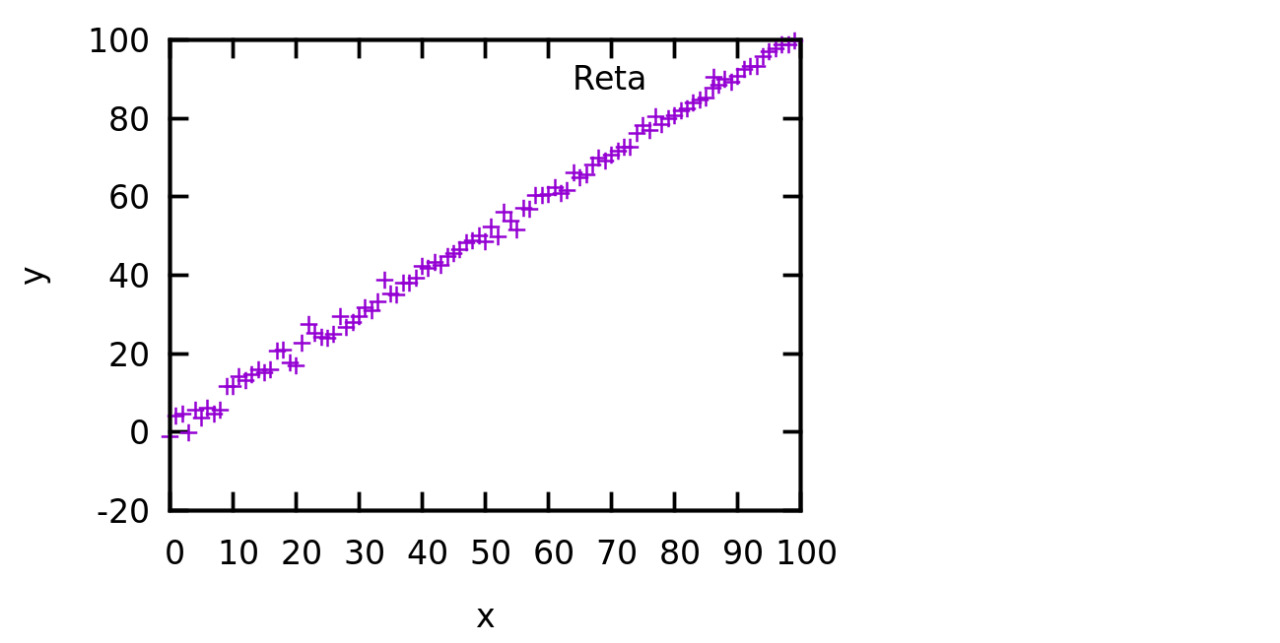
\includegraphics[width=0.8\textwidth]{Reta.jpg}
  \caption{Dados criados a partir da reta X=Y.}
  \end{figure}
  \end{itemize}
  \end{frame}
  
  \begin{frame}{Aplicação}
  \begin{itemize}
  \item \textbf{Função Custo a cada Iteração}
  \begin{figure}
  \centering
  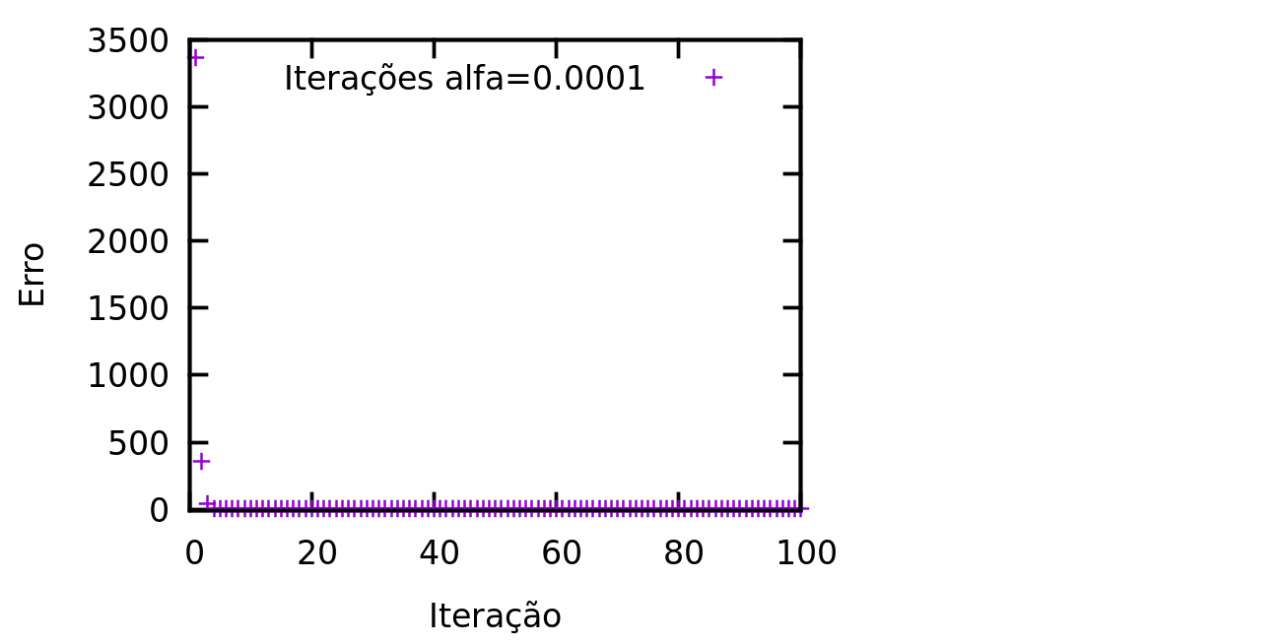
\includegraphics[width=0.8\textwidth]{custo_iteration.jpg}
  \caption{Gráfico de Custo por quantidade de iterações.}
  \end{figure}
  \end{itemize}
  \end{frame}
  
  \begin{frame}{Aplicação}
  \begin{itemize}
  \item \textbf{Resultado Final}
  \begin{figure}
  \centering
  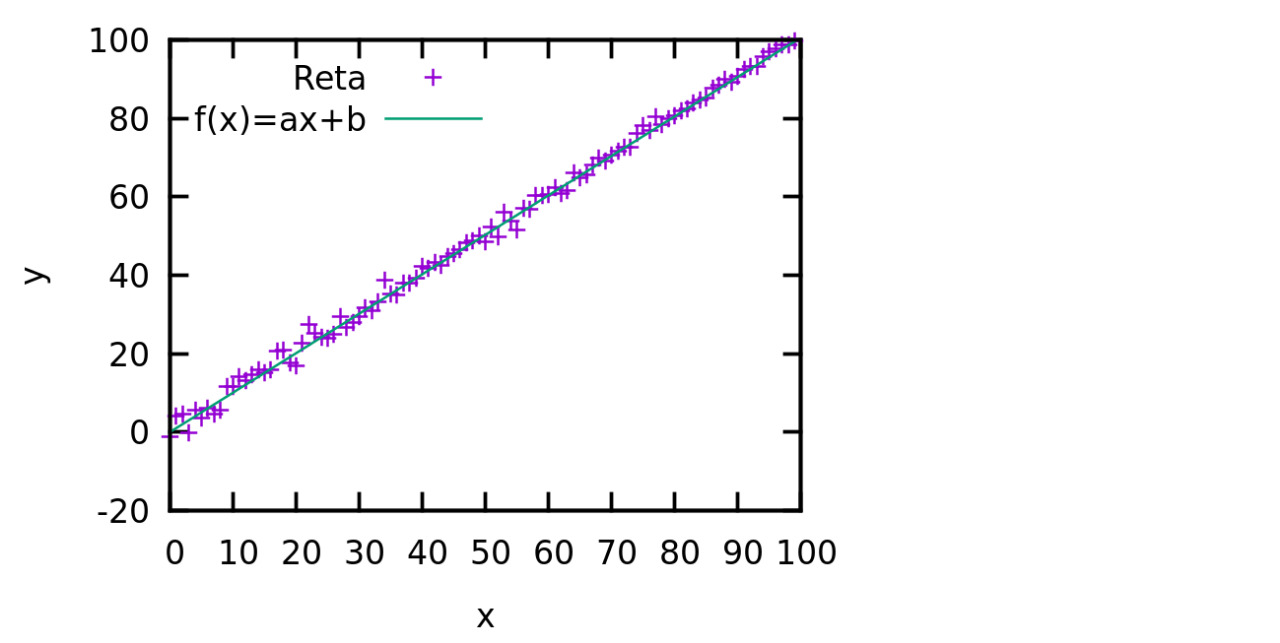
\includegraphics[width=0.8\textwidth]{reta_f_x_.jpg}
  \caption{Gráfico da Reta obtida analiticamente de coeficiente angular a = 1.00 e coeficiente linear b = -0.6 criada a partir dos dados gerados.}
  \end{figure}
  \end{itemize}  
  \end{frame}
  
    \begin{frame}{Aplicação}
  \begin{figure}
  \centering
  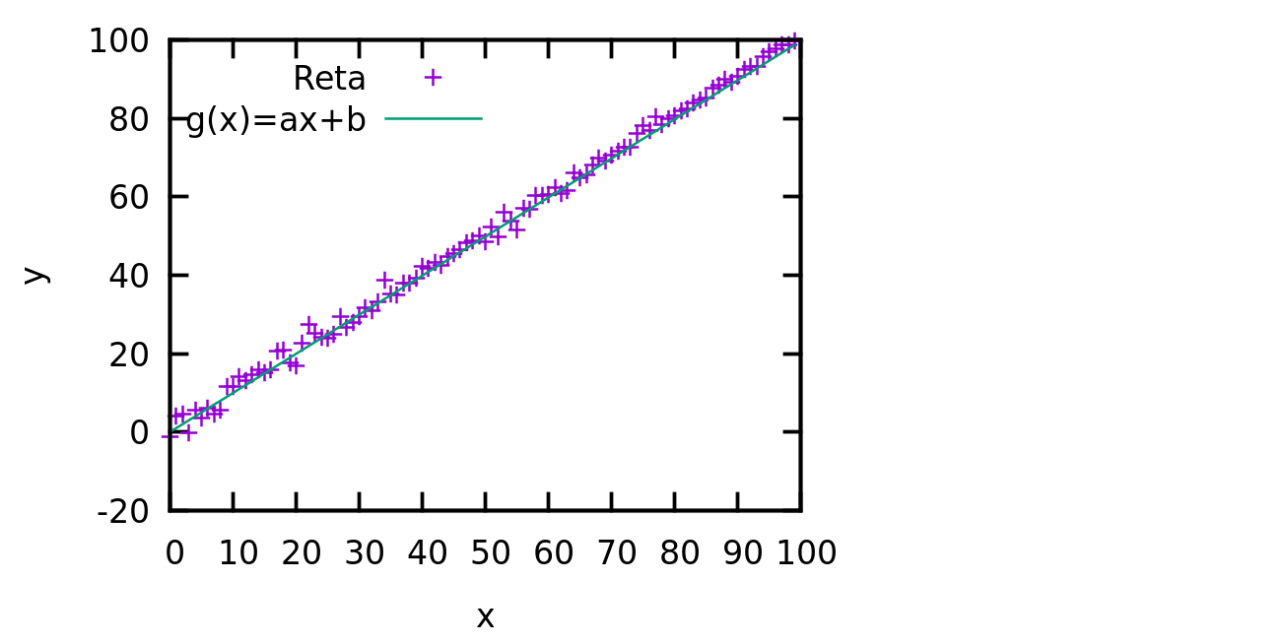
\includegraphics[width=0.8\textwidth]{reta_g_x_.jpg}
  \caption{Gráfico da Reta obtida numericamente de coeficiente angular a=0.99 e coeficiente linear b = 0.01 criada a partir dos dados gerados.}
  \end{figure}
  \end{frame}
  
  \begin{frame}{Regressão Logística}
  \begin{itemize}
  \item \textbf{Classificação}
  
  A classificação é um problema de regressão que associa a cada valor da amostra um valor discreto. Neste caso vamos analisar para classificação binária (Positivo ou Negativo, 0 ou 1, -1 ou 1, etc). 
  \item \textbf{Regressão Logística}
  
  O método de regressão logística utiliza a probabilidade de um determinado dado da amostra ser classificado por dos um valores discretos. A hipótese da regressão logística é que a probabilidade pode ser descrita como uma função logística (Sigmoid Function) que é dada por:
 
 \begin{equation}
 	h_w(X^{(i)}) = \frac{1}{1 + e^{-X^{(i)}W^T}}
 \end{equation}
 \end{itemize}
  \end{frame}
  
  \begin{frame}{Regressão Logística}
  \begin{itemize}
  \item \textbf{Sigmoid Function}
  
  \begin{figure}
  \centering 
  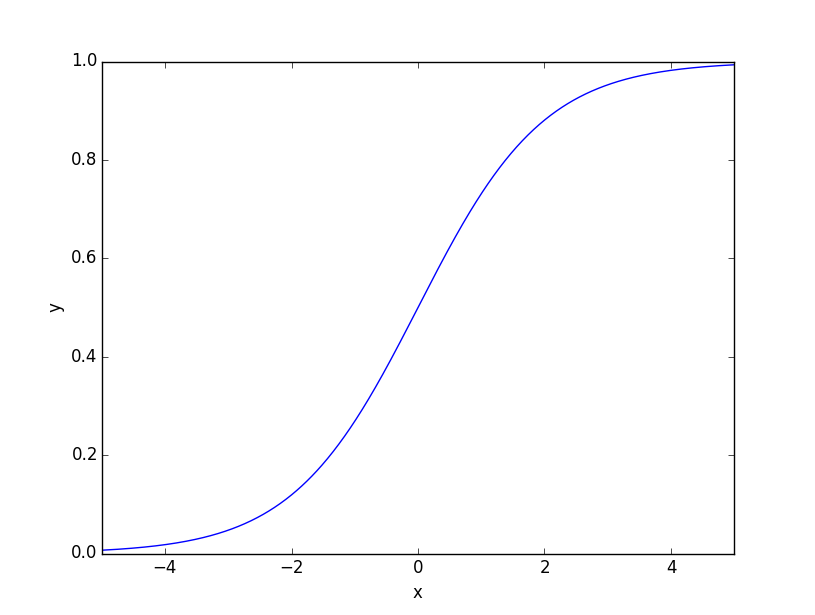
\includegraphics[width=0.6\textwidth]{sigmoid.png}
  \end{figure}
  O comportamento da função é tal que a função tende a 1 quando x $\rightarrow \infty$ e quando x $\rightarrow -\infty$  a função tende a zero.
  \end{itemize}
  \end{frame}
  
  \begin{frame}{Regressão Logística}
  \begin{itemize}
  \item \textbf{Método do Gradiente Decrescente}
  
  Para utilizar essa técnica já descrita anteriormente é necessário o cálculo da derivada de $h_W(X^{(i)})$. Então, $h^{'}(W)$ é dada por:
  \begin{equation}
  \begin{split}
  \frac{d}{dW}h_W (X^{(i)}) = \frac{d}{dW} =\frac{1}{1 + e^{-X^{(i)}W^T}} = \frac{1}{1 + e^{-X^{(i)}W^T}}(e^{-X^{(i)}W^T})\\
  = \frac{1}{1 + e^{-X^{(i)}W^T}}\left( 1 - \frac{1}{1 + e^{X^{(i)}W^T}} \right) = h_W(X^{(i)})(1 - h_W(X^{(i)}))
  \end{split}
  \end{equation}
  
  Assim, de maneira semelhante ao modelo de Regressão Linear em que é adotado um conjunto de superposições de vetores derivadas, aqui é possível utilizar superposições probabilísticas a fim de maximizar o likelihood. Assumindo que a probabilidade de dado um $X^{(i)}$ e um vetor normal à hipótese ser classificado com o valor 1 é $h(W)$ e que a probabilidade dos mesmos vetor normal e $X^{(i)}$ ser classificado com o valor 0 é 1 \- $h(W)$. 
   \end{itemize}
   \end{frame}

   
  \begin{frame}{Regressão Logística}
  \begin{itemize}
  \item Likelihood
  
   Ou seja,
  \begin{equation*}
  P(Y^{(i)} = 1 | X^{(i)},W) =  h_W (X^{(i)})
  \end{equation*}
  \begin{equation*}
    P(Y^{(i)} = 0 | X^{(i)},W) = 1 - h_W (X^{(i)})
  \end{equation*}
  Essa configuração de probabilidade condicional pode ser escrita de maneira mais funcional como:
  \begin{equation}
  p(Y^{(i)}|X^{(i)},W) = (h_W(X^{(i)}))^{Y^{(i)}}(1 - h_W(X^{(i)}))^{1-Y^{(i)}}
  \end{equation}
  Assim,a probabilidade para um número N de amostras IID é dada pela multiplicação de todas as probabilidades individuais.  
  \end{itemize}
  \end{frame}
  
  \begin{frame}{Regressão Logística}
  \begin{itemize}
  \item Likelihood
	
    Ou seja:
    \begin{equation}
    L(W) = \prod_{i = 1}^N (h_W(X^{(i)}))^{Y^{(i)}}(1 - h_W(X^{(i)}))^{1-Y^{(i)}}
    \end{equation}
    Assim como na interpretação probabilística da Regressão Linear, é necessário maximizar o log(L(W)):
    \begin{equation}
   \sum_{i=1}^N Y^{(i)} \log h_W(X^{(i)}) + (1 - Y^{(i)}) \log( 1 - h_W(X^{(i)}))
    \end{equation}
    Então, derivando:
    \begin{equation}
    \frac{\partial }{\partial W} l(W) = \left( \frac{y}{h_W(X^{(i)})} - (1 - y)\frac{1}{1 - h_W(X^{(i)})}\right) \frac{\partial}{\partial W} h_W(X^{(i)})
    \end{equation}    
  \end{itemize}
  \end{frame}
  
  \begin{frame}{Regressão Logística}
  \begin{itemize}
  \item Likelihood
  \begin{equation}
  \frac{\partial }{\partial W} l(W) = (Y^{(i)} - h_W(X^{(i)})) X^{(i)}
  \end{equation}
  Assim, o método do gradiente crescente:
  \begin{equation}
  W_{t+1} = W_t + \alpha (Y^{(i)} - h_W(X^{(i)}))X^{(i)}
  \end{equation}
  \end{itemize}
  \end{frame}
  
  \begin{frame}{Resultados}
 	\begin{figure}
 	\centering
    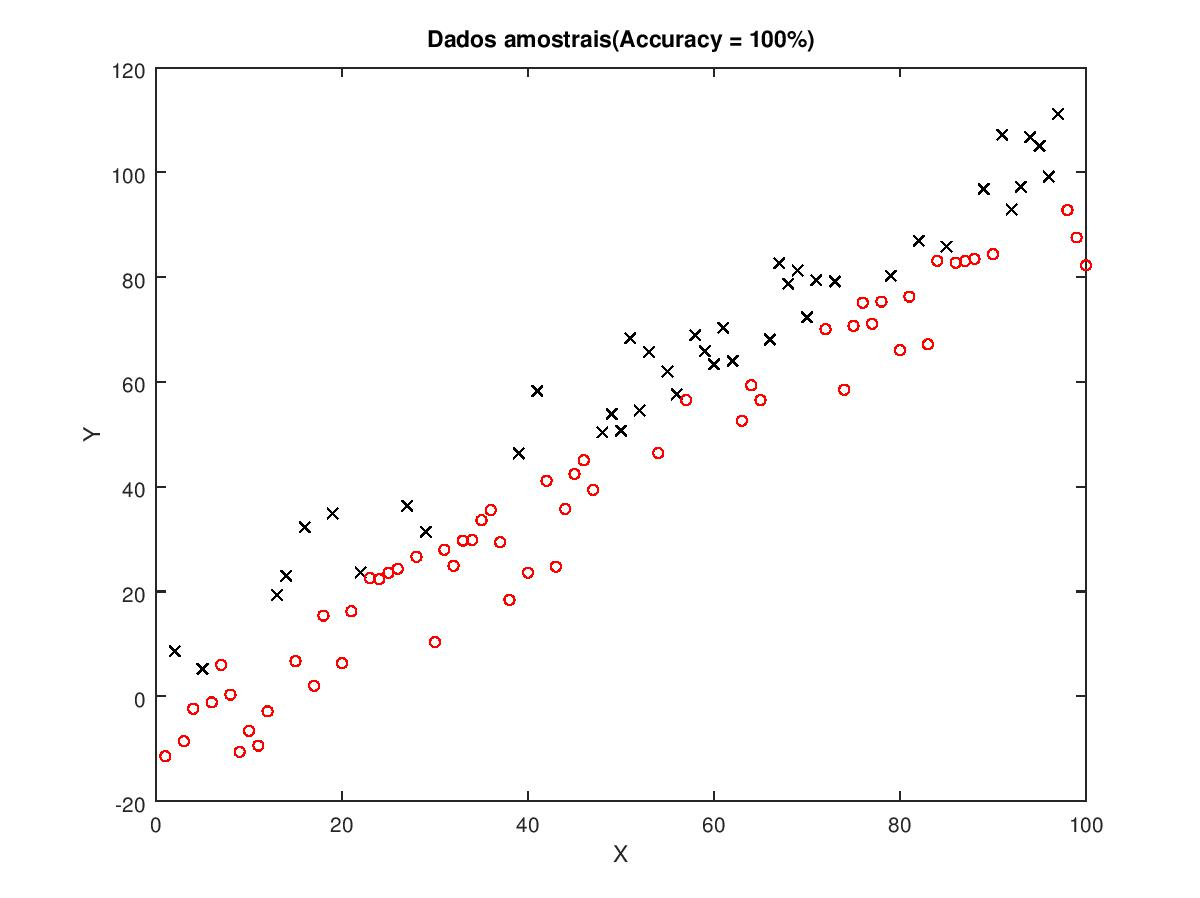
\includegraphics[width= 0.8\textwidth]{Amostra.jpg}
   \caption{Dados Amostrais classificados por valores binário(0,1), acima da reta é classificado por 1 e abaixo por 0. }
 	\end{figure}
  \end{frame}
  \begin{frame}{Resultdos}
  \begin{figure}
  \centering
  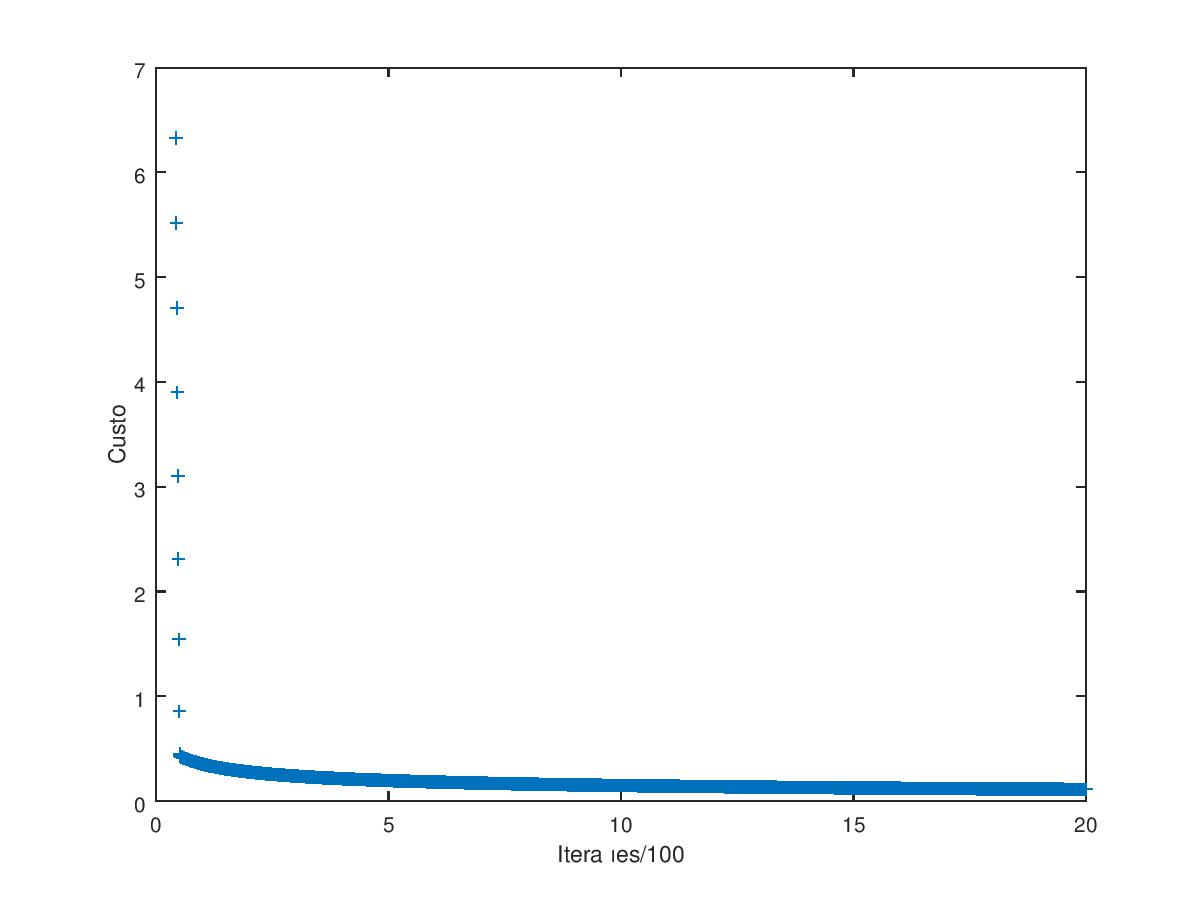
\includegraphics[width=0.8\textwidth]{Custo.jpg}
  \caption{Valores do custo em função do número de iteração.}  \end{figure}
  \end{frame}
  \begin{frame}{Resultados}
  \begin{figure}
  \centering
  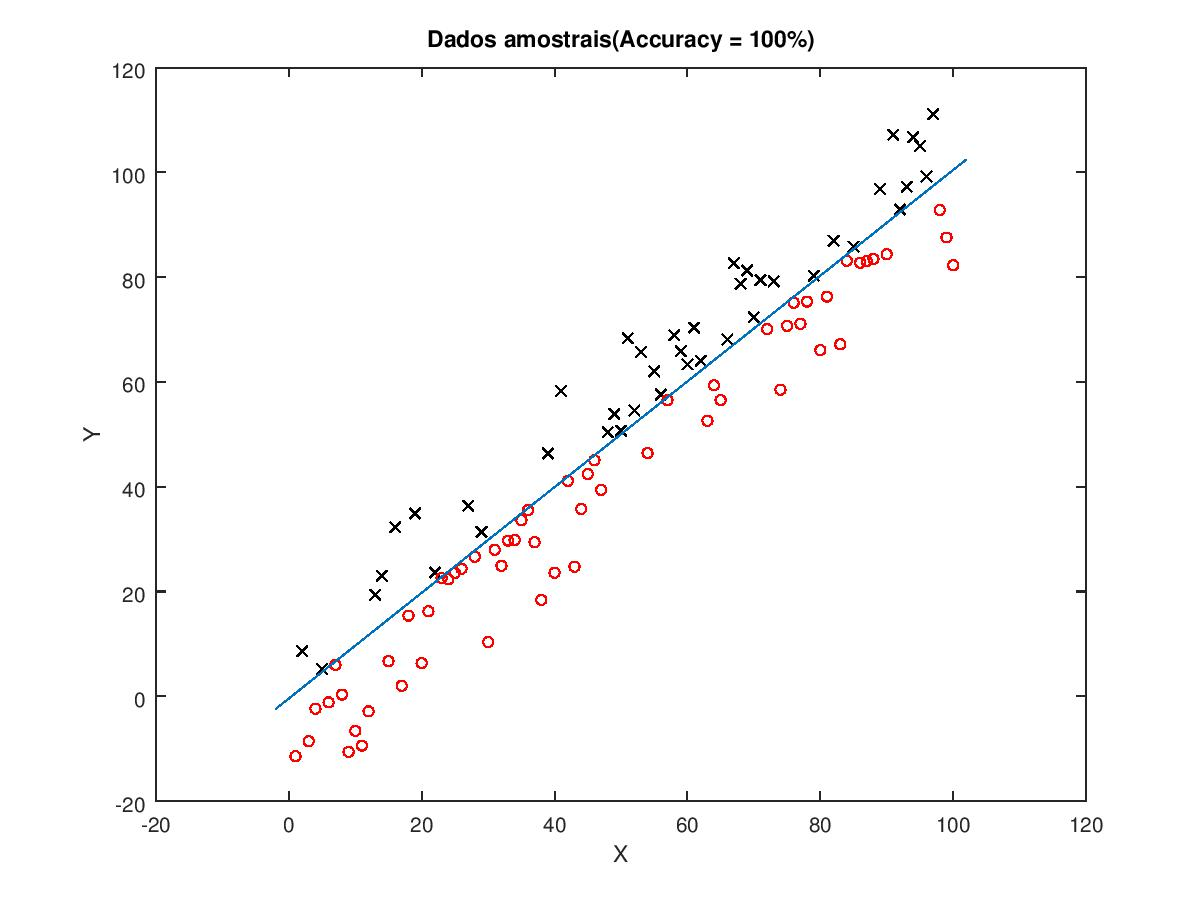
\includegraphics[width=0.8\textwidth]{General.jpg}
  \caption{Amostra e Reta de decisão obtida após a implementação.}
  \end{figure}
  \end{frame}
  \begin{frame}{Referências}
   [1]	http://www.portalaction.com.br/analise-de-regressao. Acessado em 04/05/2018.
   
   [2] https://www.researchgate.net/figure/A-plot-of-the-gradient-descent-algorithm-left-and-the-stochastic-gradient-descent\_fig1\_303257470. Acessado em 04/05/2018.
  \end{frame}
\end{document}
